\documentclass{beamer}
%pdflatex -shell-escape my_document.tex

\usetheme{default}
\usecolortheme{rose}
\usefonttheme{serif}
%\usefonttheme{structureitalicsserif}

\definecolor{verdeuni}{rgb}{0.7,0.73437,0.55856}
\setbeamertemplate{headline}[verdeuni]
%\setbeamercovered{highly dinamic}
%\usepackage{eso-pic}

\usepackage{minted}

\usepackage{stmaryrd}
\usepackage{local-macros2}
\newcommand{\distance}[2]{|#1 - #2|}
\newcommand{\outputdistance}[2]{||#1 - #2||}
%\newcommand{\x}{\vect{x}} 		% Arbitrary input
%\newcommand{\xt}{\hat{\x}} 		% Training input
\newcommand{\xs}{\x} 			% Sampled input
\newcommand{\xp}{\tilde{\x}} 	% Perturbed input

%\newcommand{\y}{\vect{y}} 		% Arbitrary output
\newcommand{\yt}{\hat{\y}} 		% Training output
\newcommand{\ys}{\y} 			% Sampled output



\newcommand{\SR}[2]{SR(#1, #2)} % Standard robustness
\newcommand{\LR}[2]{LR(#1, #2)} % Lipschitz robustness
\newcommand{\CR}[1]{CR(#1)} % Classification robustness
\newcommand{\SCR}[2]{SCR(#1,#2)} % Approximate class. robustness

\usepackage{amsfonts,amsmath,amssymb,amsthm}
\usepackage[all]{xy}
\usepackage{array,url}
\usepackage{textcomp,textgreek}
\usepackage{pgfplots}
\usepackage{float}
\pgfplotsset{width=5cm,compat=1.9}
\usepackage{mdframed,wrapfig,subcaption}
%\usepackage[font=footnotesize,labelfont=it
%\usepackage[latin1]{inputenc}
\usepackage{babel}
\usepackage{color}
%\usepackage{url}
\usepackage{hyperref}
\usepackage{fancyvrb}
%\usepackage{tikz}
\usepackage{alltt}
%\usepackage{etex, xy}
%\usepackage{cibeamer}
\usepackage{tikz}
\usetikzlibrary{arrows,shapes}
%\xyoption{all}
%\usepackage{listings}
%\input macro
\usepackage{cancel, comment}
\usepackage{verbatim}
\usepackage{slashbox}
\usepackage{ulem}

\newcommand{\tikzmark}[1]{\tikz[remember picture] \node[coordinate] (#1) {#1};}
\newcommand{\semitransp}[2][35]{\color{fg!#1}#2}

\usepackage[absolute,overlay]{textpos}
\beamertemplatenavigationsymbolsempty
\usepackage{ijcnn-diagram}

\usepackage[all]{foreign}

\newcommand{\fstar}{F$^\ast$\xspace}
\newcommand{\starchild}{StarChild\xspace}
\newcommand{\lazuli}{Lazuli\xspace}
\newcommand{\sapphire}{Sapphire\xspace}
\newcommand{\cL}{{\cal L}}
%\newcommand{\Real}{{\mathbb R}}
\usepackage{makecell}
\DeclareMathOperator{\linear}{linear}
\DeclareMathOperator{\relu}{relu}
\DeclareMathOperator{\sigmoid}{sigmoid}
\DeclareMathOperator{\softmax}{softmax}
\DeclareMathOperator{\neuron}{neuron}
\DeclareMathOperator{\truthy}{truthy}
\DeclareMathOperator{\falsey}{falsey}
\DeclareMathOperator{\neurontest}{test}
\usepackage{ellipsis}
\renewcommand{\ellipsisgap}{-0.25em}

\usepackage{soul}
\makeatletter
\let\HL\hl
\renewcommand\hl{%
  \let\set@color\beamerorig@set@color
  \let\reset@color\beamerorig@reset@color
  \HL}
\makeatother

%\usetikzlibrary{decorations.pathreplacing,shapes.arrows}
\newcommand\BackgroundPicture[1]{%
  \setbeamertemplate{background}{%
   \parbox[c][\paperheight]{\paperwidth}{%
      \vfill \hfill
\includegraphics[width=1\paperwidth,height=1\paperheight]{#1}
        \hfill \vfill
     }}}
\usepackage{xcolor,colortbl}
%\usepackage{listings}
\definecolor{Gray}{gray}{0.85}

%\setbeamertemplate{footline}[frame number]

%\newcommand{\rrdc}{\mbox{\,\(\Rightarrow\hspace{-9pt}\Rightarrow\)\,}} % Right reduction
%\newcommand{\lrdc}{\mbox{\,\(\Leftarrow\hspace{-9pt}\Leftarrow\)\,}}% Left reduction
%\newcommand{\lrrdc}{\mbox{\,\(\Leftarrow\hspace{-9pt}\Leftarrow\hspace{-5pt}\Rightarrow\hspace{-9pt}\Rightarrow\)\,}} % Equivalence
%\DeclareMathOperator{\id}{Id}
%\newcommand{\Zset}{\mathbb{Z}}
%\newcommand{\Bset}{\mathbb{Z}_2}

\setbeamertemplate{navigation symbols}{}

\mode<presentation>
\title[Vehicle Tutorial Introduction]{Neural Network Verification with Vehicle}
%\subtitle{in Neuro-Symbolic Landscape}
\author[Vehicle]{Ekaterina Komendantskaya and Matthew Daggitt (today's presentors), on behalf of the Vehicle team}
\institute[]{}

\date[]{}

%\logo{
\includegraphics[width=6cm]{LaivLogolong.png}}

\AtBeginSection[]
{
  \begin{frame}
    \frametitle{Table of Contents}
    \tableofcontents[currentsection]
  \end{frame}
}

\begin{document}
\BackgroundPicture{logo1.png}

\begin{frame}
\titlepage
\end{frame}

\begin{frame}
  \frametitle{The Vehicle Team}

%\begin{center}
%  \includegraphics[width=7cm]{DSC_2635.jpg}
%\end{center}
 \begin{columns}
   \column{.3\textwidth}
   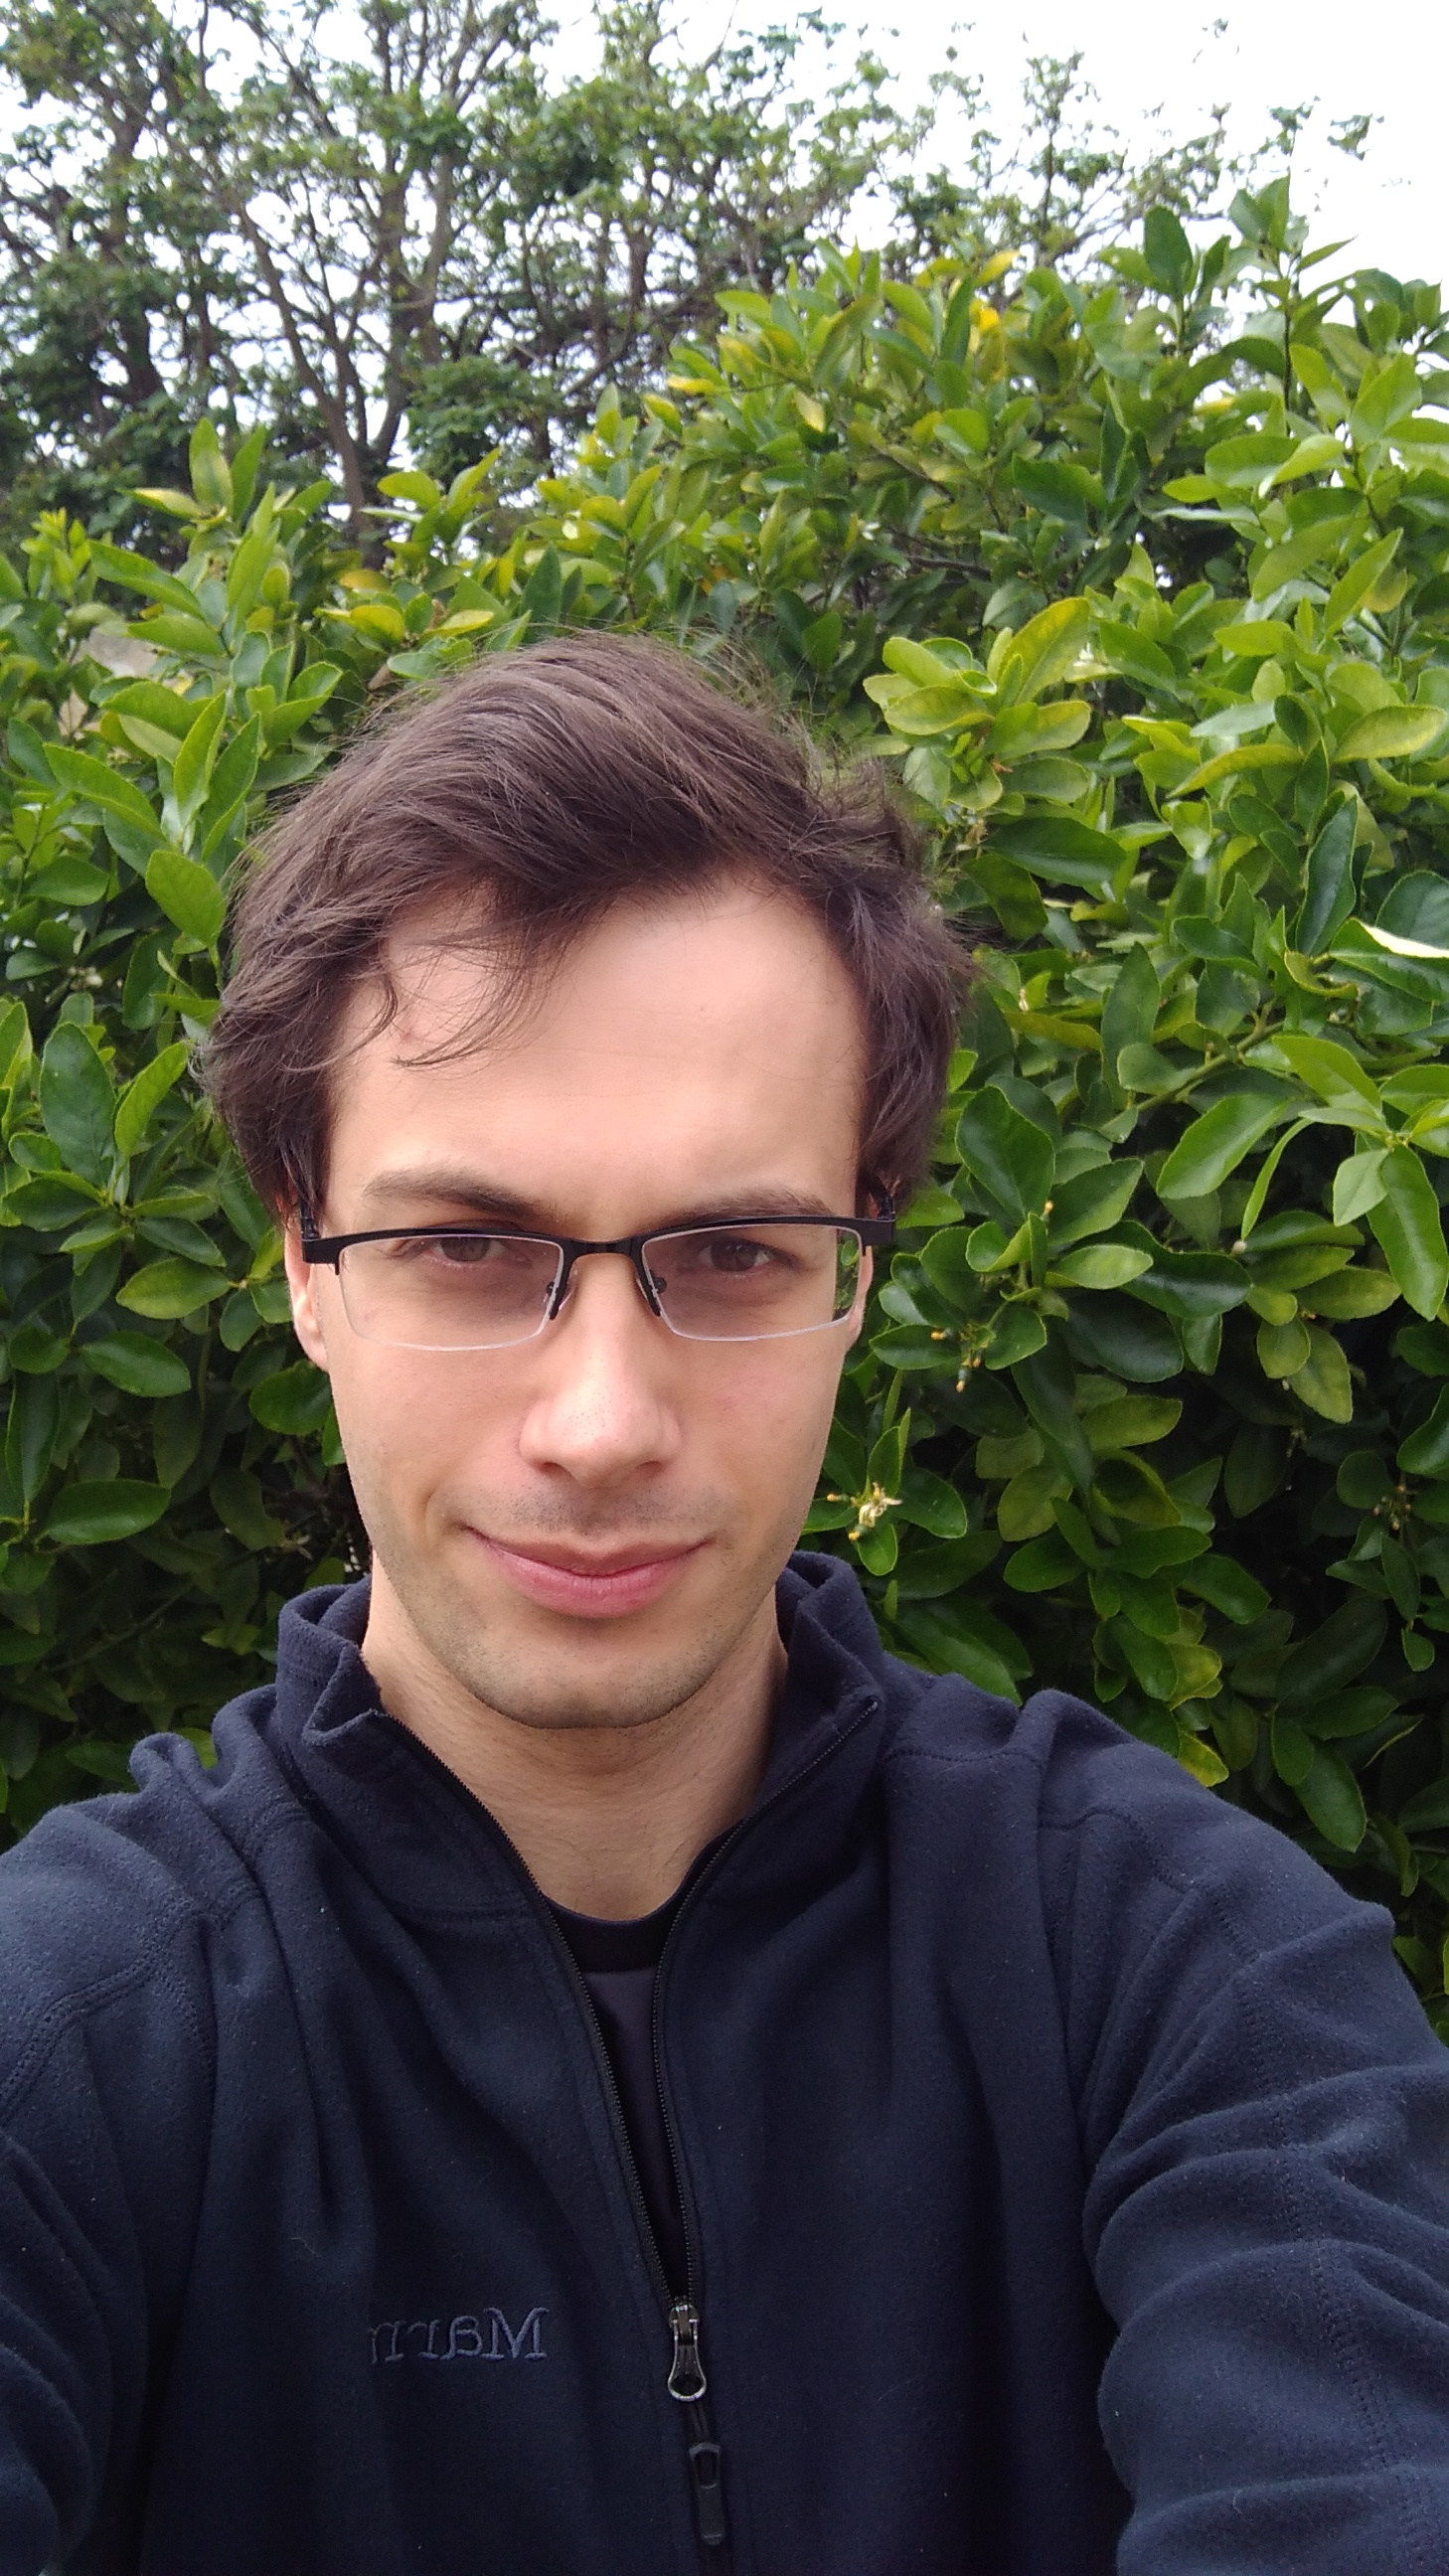
\includegraphics[width=1.3cm]{Images/Matthew.jpg}

      \begin{alertblock}{\footnotesize{Matthew Daggitt}}
     \end{alertblock}
    
          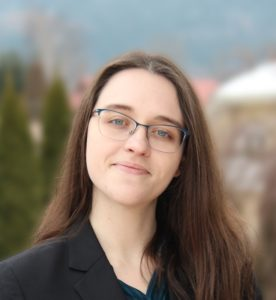
\includegraphics[width=1.5cm]{Images/Natalia.jpg}
           \begin{block}{\footnotesize{Natalia Slusarz}}
           \end{block}
           
           
\includegraphics[width=1.5cm]{Images/Ben.jpg}
   \begin{block}{\footnotesize{Ben Coke}}
     
     \end{block}

  %\includegraphics[width=2cm]{Manuel_Maarek.jpg}

  % \includegraphics[width=2cm]{photoDP.jpg}
   \column{.3\textwidth}
   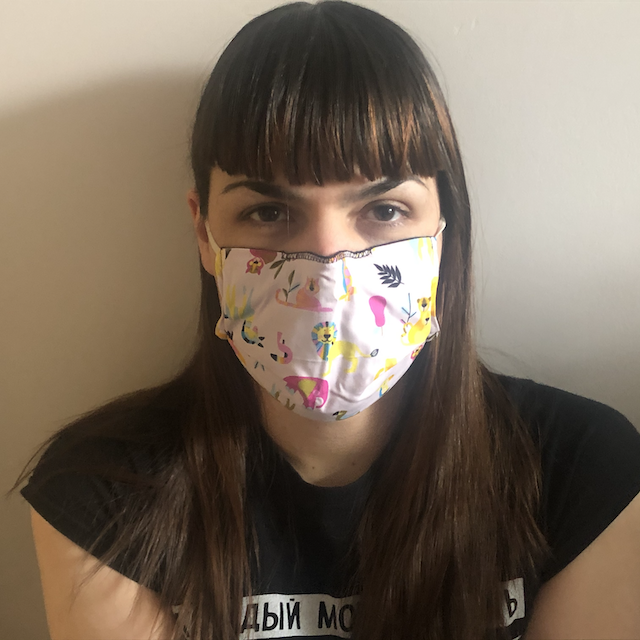
\includegraphics[width=1.6cm]{Images/Wen.png}
   \begin{alertblock}{\footnotesize{Wen Kokke}}
   \end{alertblock}
    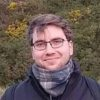
\includegraphics[width=1.8cm]{Images/Luca.jpeg}
    \begin{block}{\footnotesize{Luca Arnaboldi}}
   \end{block}
  
\includegraphics[width=1.8cm]{Images/Marco.jpg}
        \begin{block}{\footnotesize{Marco Casadio}}
     \end{block}

  %    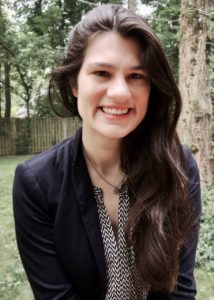
\includegraphics[width=1.5cm]{Images/Kathrin.jpg}
  %\begin{block}{\footnotesize{Kathrin Stark}}
  % \end{block}


   \column{.3\textwidth}

     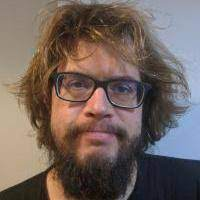
\includegraphics[width=1.6cm]{Images/Bob.jpeg}

         % \includegraphics[width=2cm]{photoDP.jpg}
          \begin{block}{\footnotesize{Bob Atkey}}
     \end{block}

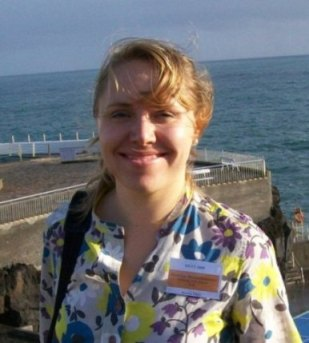
\includegraphics[width=1.8cm]{Images/Katya3.jpg}
\begin{block}{\footnotesize{Katya K}}
   \end{block}


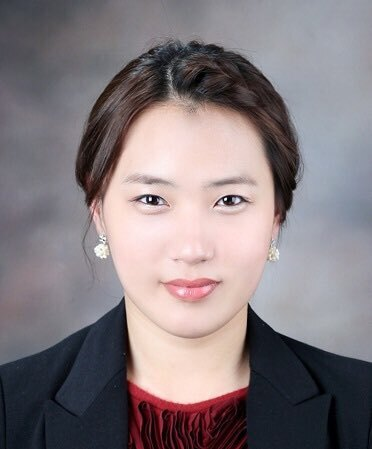
\includegraphics[width=1.8cm]{Images/JL.jpeg}
\begin{block}{\footnotesize{Jeonghyeon Lee}}
   \end{block}
    
   
  \end{columns}
  \end{frame}




\section{Neural Network Verification: overview of the new domain}


\begin{frame}
\frametitle{Neural nets for classification}
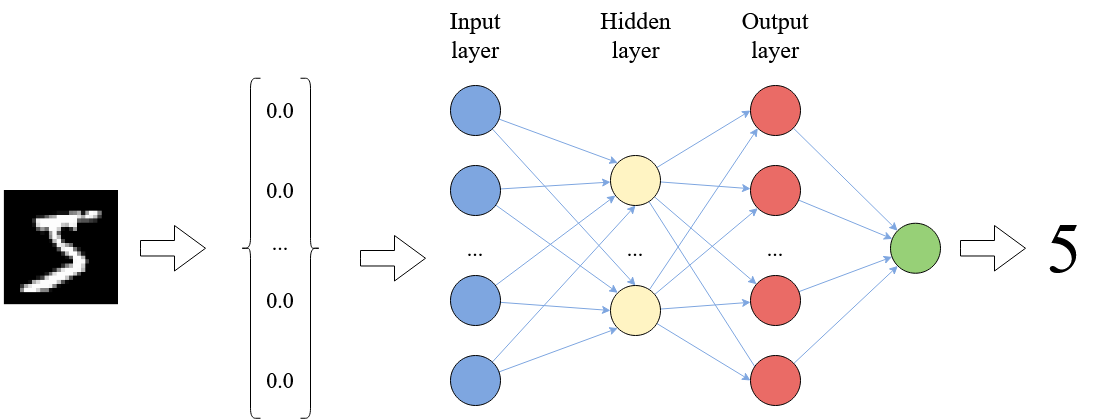
\includegraphics[scale=.30]{Images/mnist_classification.png}

\begin{block}{Formally,}
 a neural network is a function $N : R^n \rightarrow R^m$.
\end{block}

\end{frame}

\begin{frame}
\frametitle{Neural networks}

\begin{alertblock}{... are ideal for  ``perception'' tasks:}
    \setbeamercovered{transparent}
\begin{itemize}[<+->]
  \item approximate functions when exact solution is hard to get
    \item tolerant to noisy and incomplete data
    \end{itemize}
\end{alertblock}
\pause

\begin{block}{BUT}
  \begin{itemize}
   % \item continuous decision space means solutions can only be approximate
	\item solutions not easily conceptualised (\alert{lack of explainability})
	%\item prone to error
	\item prone to a new range of safety and security problems: \pause
          \begin{itemize} \item[] adversarial attacks
        \item[]  data poisoning
        \item[] catastrophic forgetting
          \end{itemize}
\end{itemize}
\end{block}
\end{frame}

\begin{frame}
  \frametitle{One example: Adversarial Attacks}

 % \begin{block}{}
 %   Given a trained neural network and a correctly classified image of ``0'' on the left,
 %                 we can create a perturbation $\eta$ (middle) to the original image so that the same neural network predicts a ``5" with 92\% confidence for the modified image (right).
 %   \end{block}

  	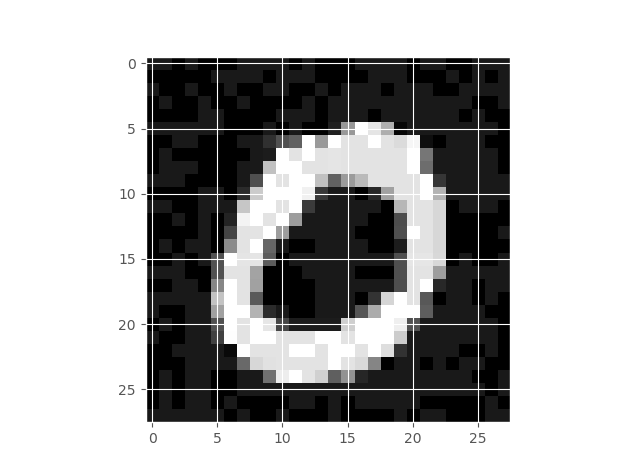
\includegraphics[width=.3\textwidth]{Images/true.png}
	\uncover<2->{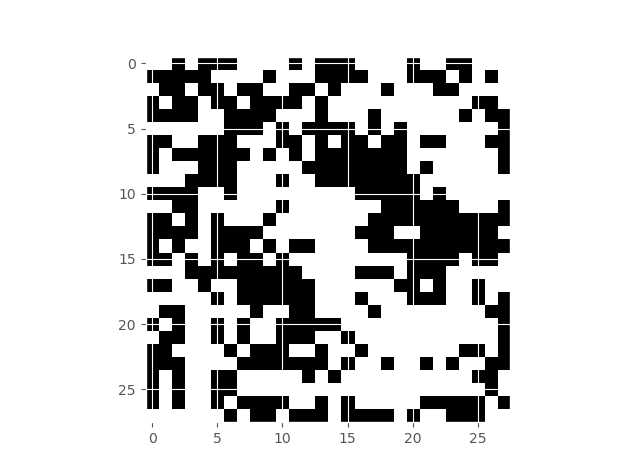
\includegraphics[width=.3\textwidth]{Images/eta.png}}
	\uncover<3->{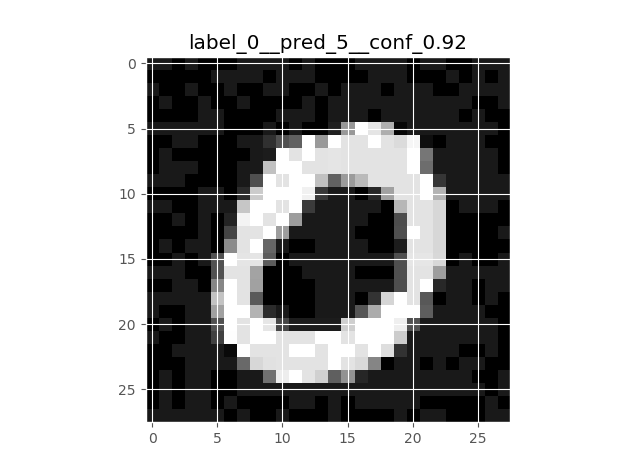
\includegraphics[width=.3\textwidth]{Images/adv.png}}

\begin{itemize}
\item<4->[] the perturbations are imperceptible to human eye \pause
\item<5->[] attacks transfer from one neural network to another \pause
\item<6->[] affect any domain where neural networks are applied
\end{itemize}

\end{frame}

\begin{frame}
      \frametitle{Verification Property:  ``$\epsilon$-ball robustness''}
\begin{center}
  \begin{tikzpicture}[scale=.8]
  % draw the sphere
  \shade[ball color = gray!40, opacity = 0.4] circle (2cm);
  \draw (0,0) circle (2cm);
  \draw (-2,0) arc (180:360:2 and 1);
  \draw[dashed] (2,0) arc (0:180:2 and 1);
  \fill[fill=black] (0,0) circle (1pt);
  \draw[dashed,<->] (0,0 ) -- node[above]{$\epsilon$} (2,0);
  % line for original image
  \draw[] (0,0 ) -- node{} (0,-2.5);
  \node (1orig) at (0,-3) {
\includegraphics{Images/7_orig.png}};
 % \node[] at (0,-3.8) {NN: ``seven''};
  % line for the perturbed image 1
  \draw[] (-0.6,1.2) -- node{} (-0.9,2.7);
  \node () at (-1,2.8) {
\includegraphics{Images/7_v1}};
  % line for the perturbed image 2
  \draw[] (0.6,1.4) -- node{} (1.2,2.7);
  \node () at (1.2,2.8) {
\includegraphics{Images/7_v2}};
  % line for the perturbed image 3
  \draw[] (0.6,-1.2) -- node{} (2.5,-2.7);
  \node () at (2.5,-2.8) {
\includegraphics{Images/7_v3}};
\end{tikzpicture}
\end{center}


  \begin{alertblock}{An $\epsilon$-ball     $\mathbb{B}(\hat{\mathbf{x}}, \epsilon) = \{ {\mathbf{x} \in \mathbb{R}^n: |\hat{\mathbf{x}}-\mathbf{x}| \leq \epsilon} \}$ }


    Classify all  points in $\mathbb{B}(\hat{\mathbf{x}}, \epsilon)$ ``robustly''.
    %in the \alert{``same class''} as $\hat{\mathbf{x}}$.
  \end{alertblock}

 % \begin{block}{}
%\end{block}
    \end{frame}


    \begin{frame}
\frametitle{Another example property: ACAS Xu}
A collision avoidance system for unmanned autonomous aircraft.
\tikz [remember picture,overlay]{
\node at ([xshift=3cm,yshift=3cm]current page.south) {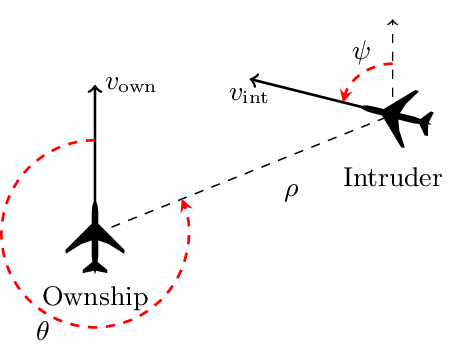
\includegraphics[width=0.5\linewidth]{Images/acas_xu.png}};}

{\small
Inputs:
\vspace{-0.7em}
\begin{itemize}
\setlength\itemsep{-0.1em}
\item Distance to intruder, $\rho$
\item Angle to intruder, $\theta$
\item Intruder heading, $\varphi$
\item Speed, $v_{own}$
\item Intruder speed, $v_{int}$
\end{itemize}


Outputs:
\vspace{-0.7em}
\begin{itemize}
\setlength\itemsep{-0.1em}
\item Clear of conflict
\item Strong left
\item Weak left
\item Weak right
\item Strong right
\end{itemize}}

\end{frame}


\begin{frame}
\frametitle{ACAS Xu}
The system was originally implemented as a 2Gb lookup table but was replaced with a neural network in order to improve size and latency requirements.

\pause
\alert{10 different specified properties in total.}

\pause
\begin{definition}[ACAS Xu: Property 1]
\emph{If the intruder is distant and is significantly slower than the ownship, the score of a COC advisory will always be below a certain fixed threshold.}
\end{definition}

\pause
\begin{block}{}
\begin{equation*}
\begin{array}{l}
(\rho \geq 55947.691) \wedge
(v_{own} \geq 1145) \wedge (v_{int} \leq 60)  \\
\Rightarrow \text{the score for COC is at most 1500}
\end{array}
\end{equation*}
\end{block}

\end{frame}

    \begin{frame}
    \frametitle{More Generally}

    \begin{block}{Given $N : R^n \rightarrow R^m$}
    Verification of such functions most commonly boils down to specifying admissible intervals for the function's output given an interval for its inputs.
\end{block}
  \uncover<2->{
    {\footnotesize
 \begin{thebibliography}{99}
 \beamertemplatearticlebibitems
\bibitem{1}{Casadio, M., Komendantskaya, E., Daggitt, M.L., Kokke, W., Katz, G., Amir, G., Refaeli, I.:
Neural network robustness as a verification property: A principled case study. In: Computer
Aided Verification (CAV 2022).}
 \end{thebibliography}}}

    \end{frame}

\begin{frame}{Overview of The Verification Landscape}%{Problem Statement}
% \centering<1>\includegraphics[width=0.8\textwidth]{img/first-slide-2015.pdf}
% \centering<2>\includegraphics[width=0.8\textwidth]{img/first-slide-2017.pdf}
% \centering<3>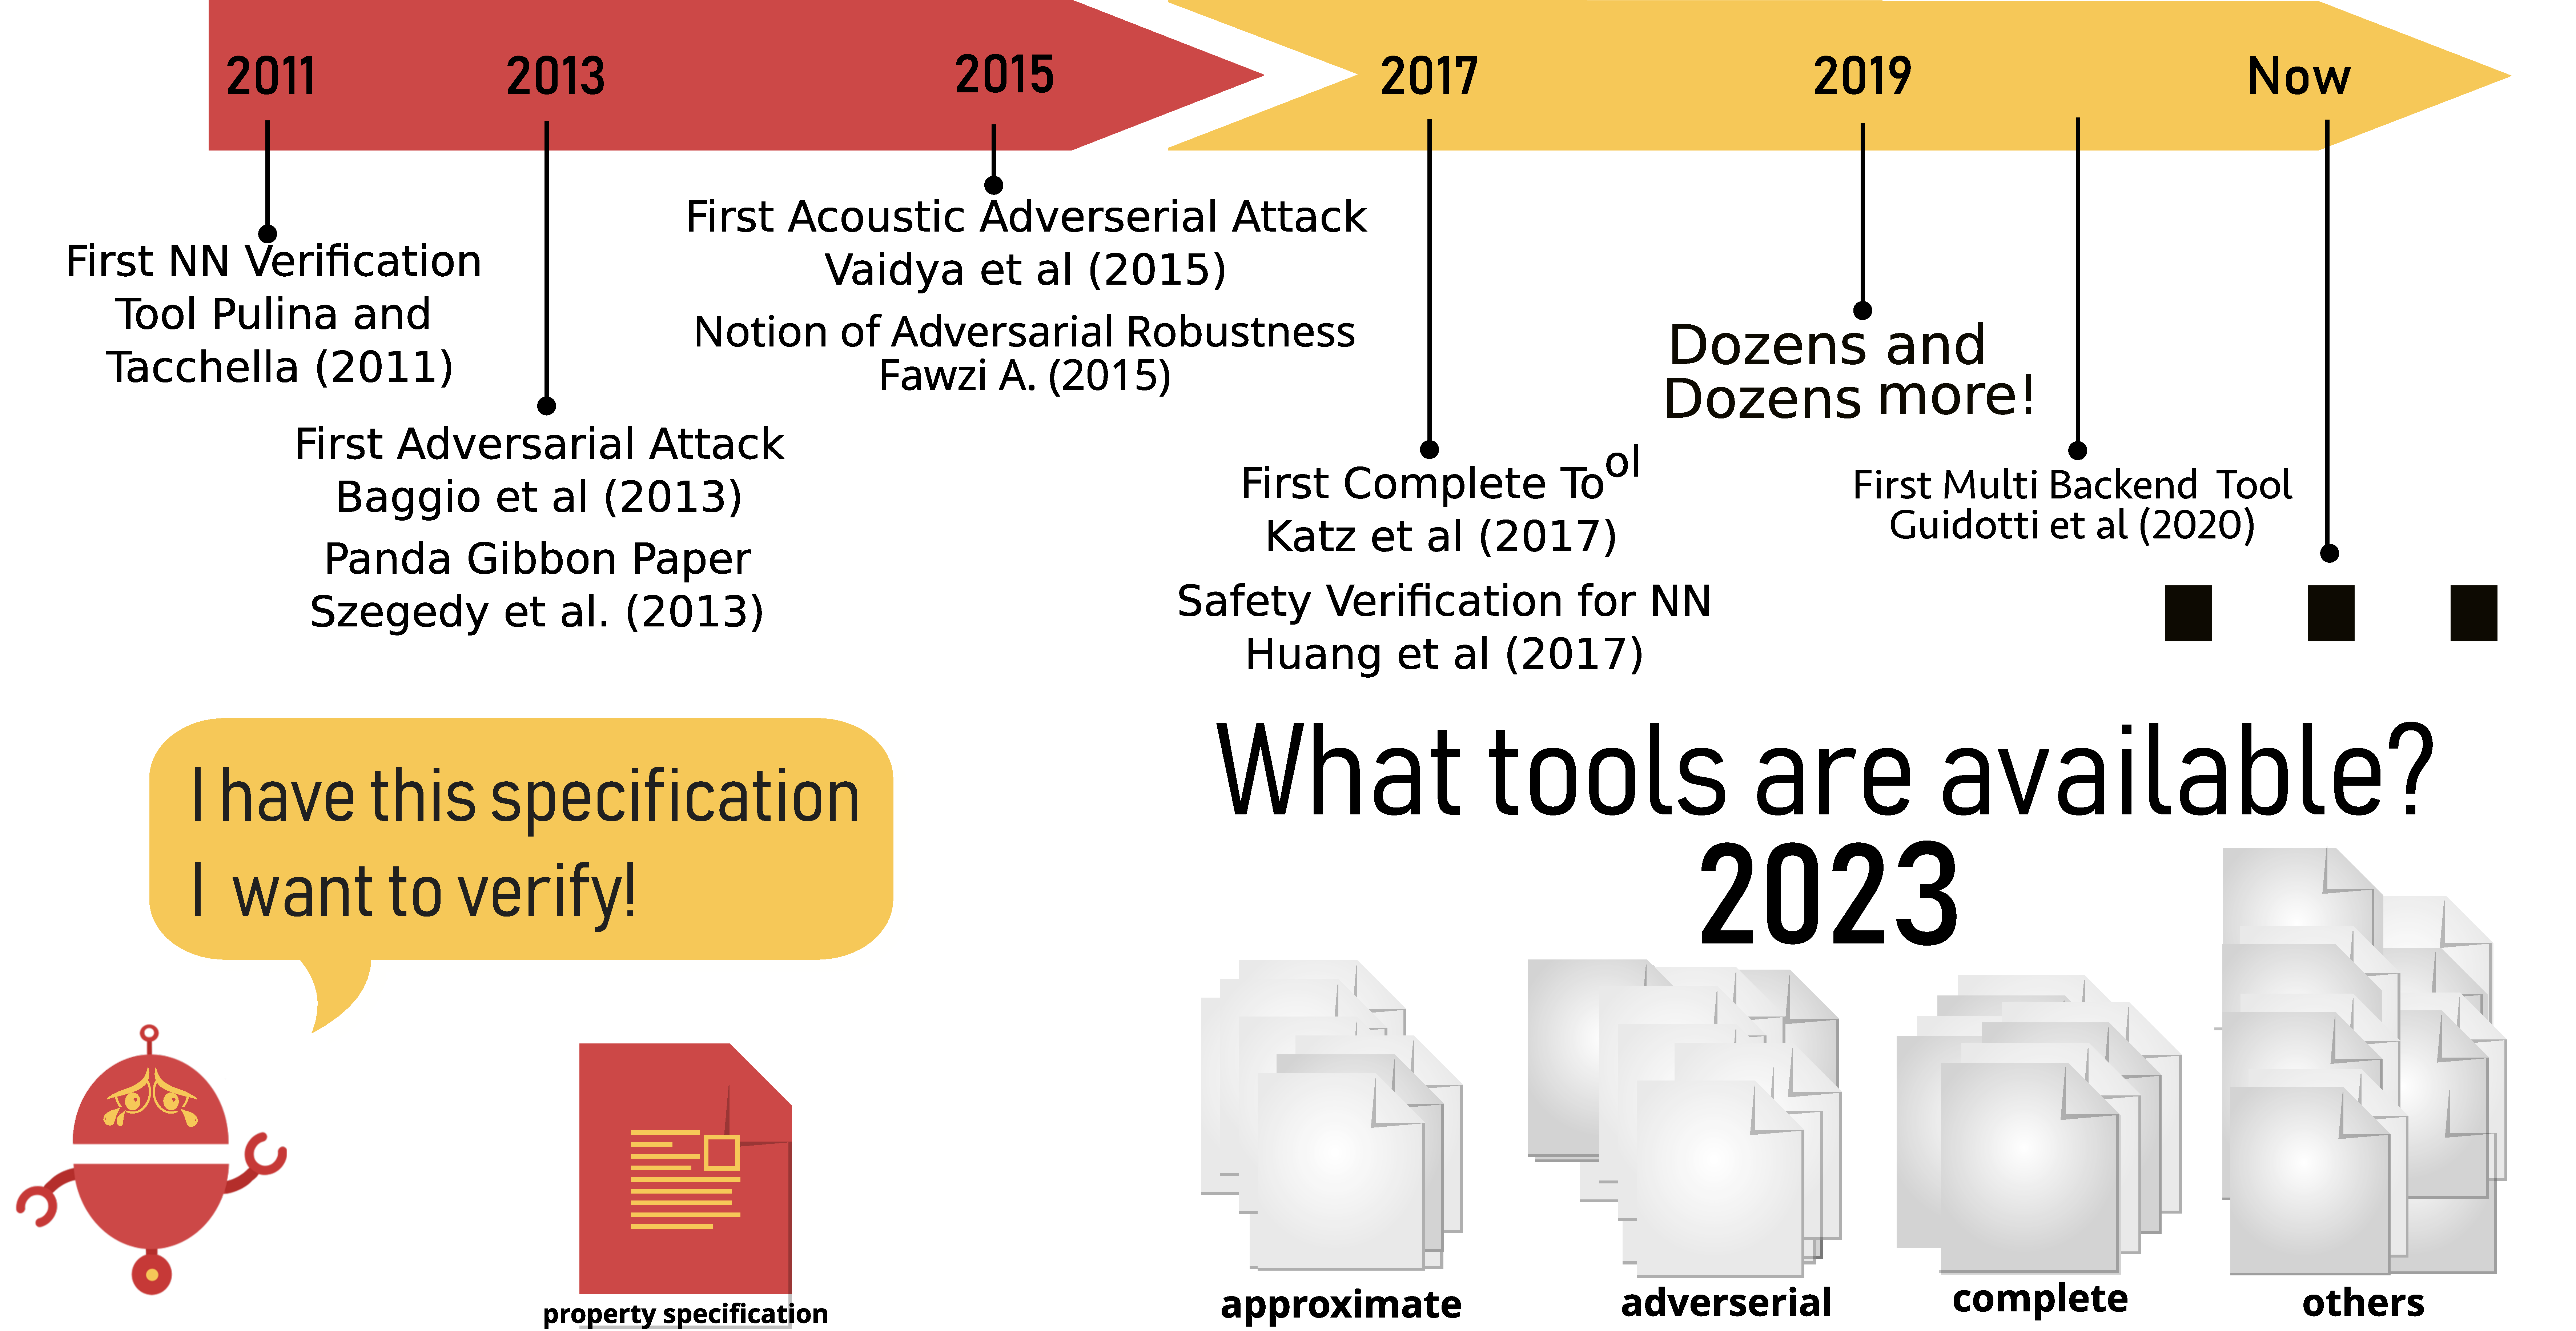
\includegraphics[width=0.8\textwidth]{img/first-slide-2022.pdf}
\only<1>{\vspace{-0.5cm}\centering\includegraphics[width=0.9\textwidth]{Images/first-slide-2015.pdf}}
\only<2>{\vspace{-0.5cm}\centering\includegraphics[width=0.9\textwidth]{Images/first-slide-2017.pdf}}
\only<3>{\vspace{-0.5cm}\centering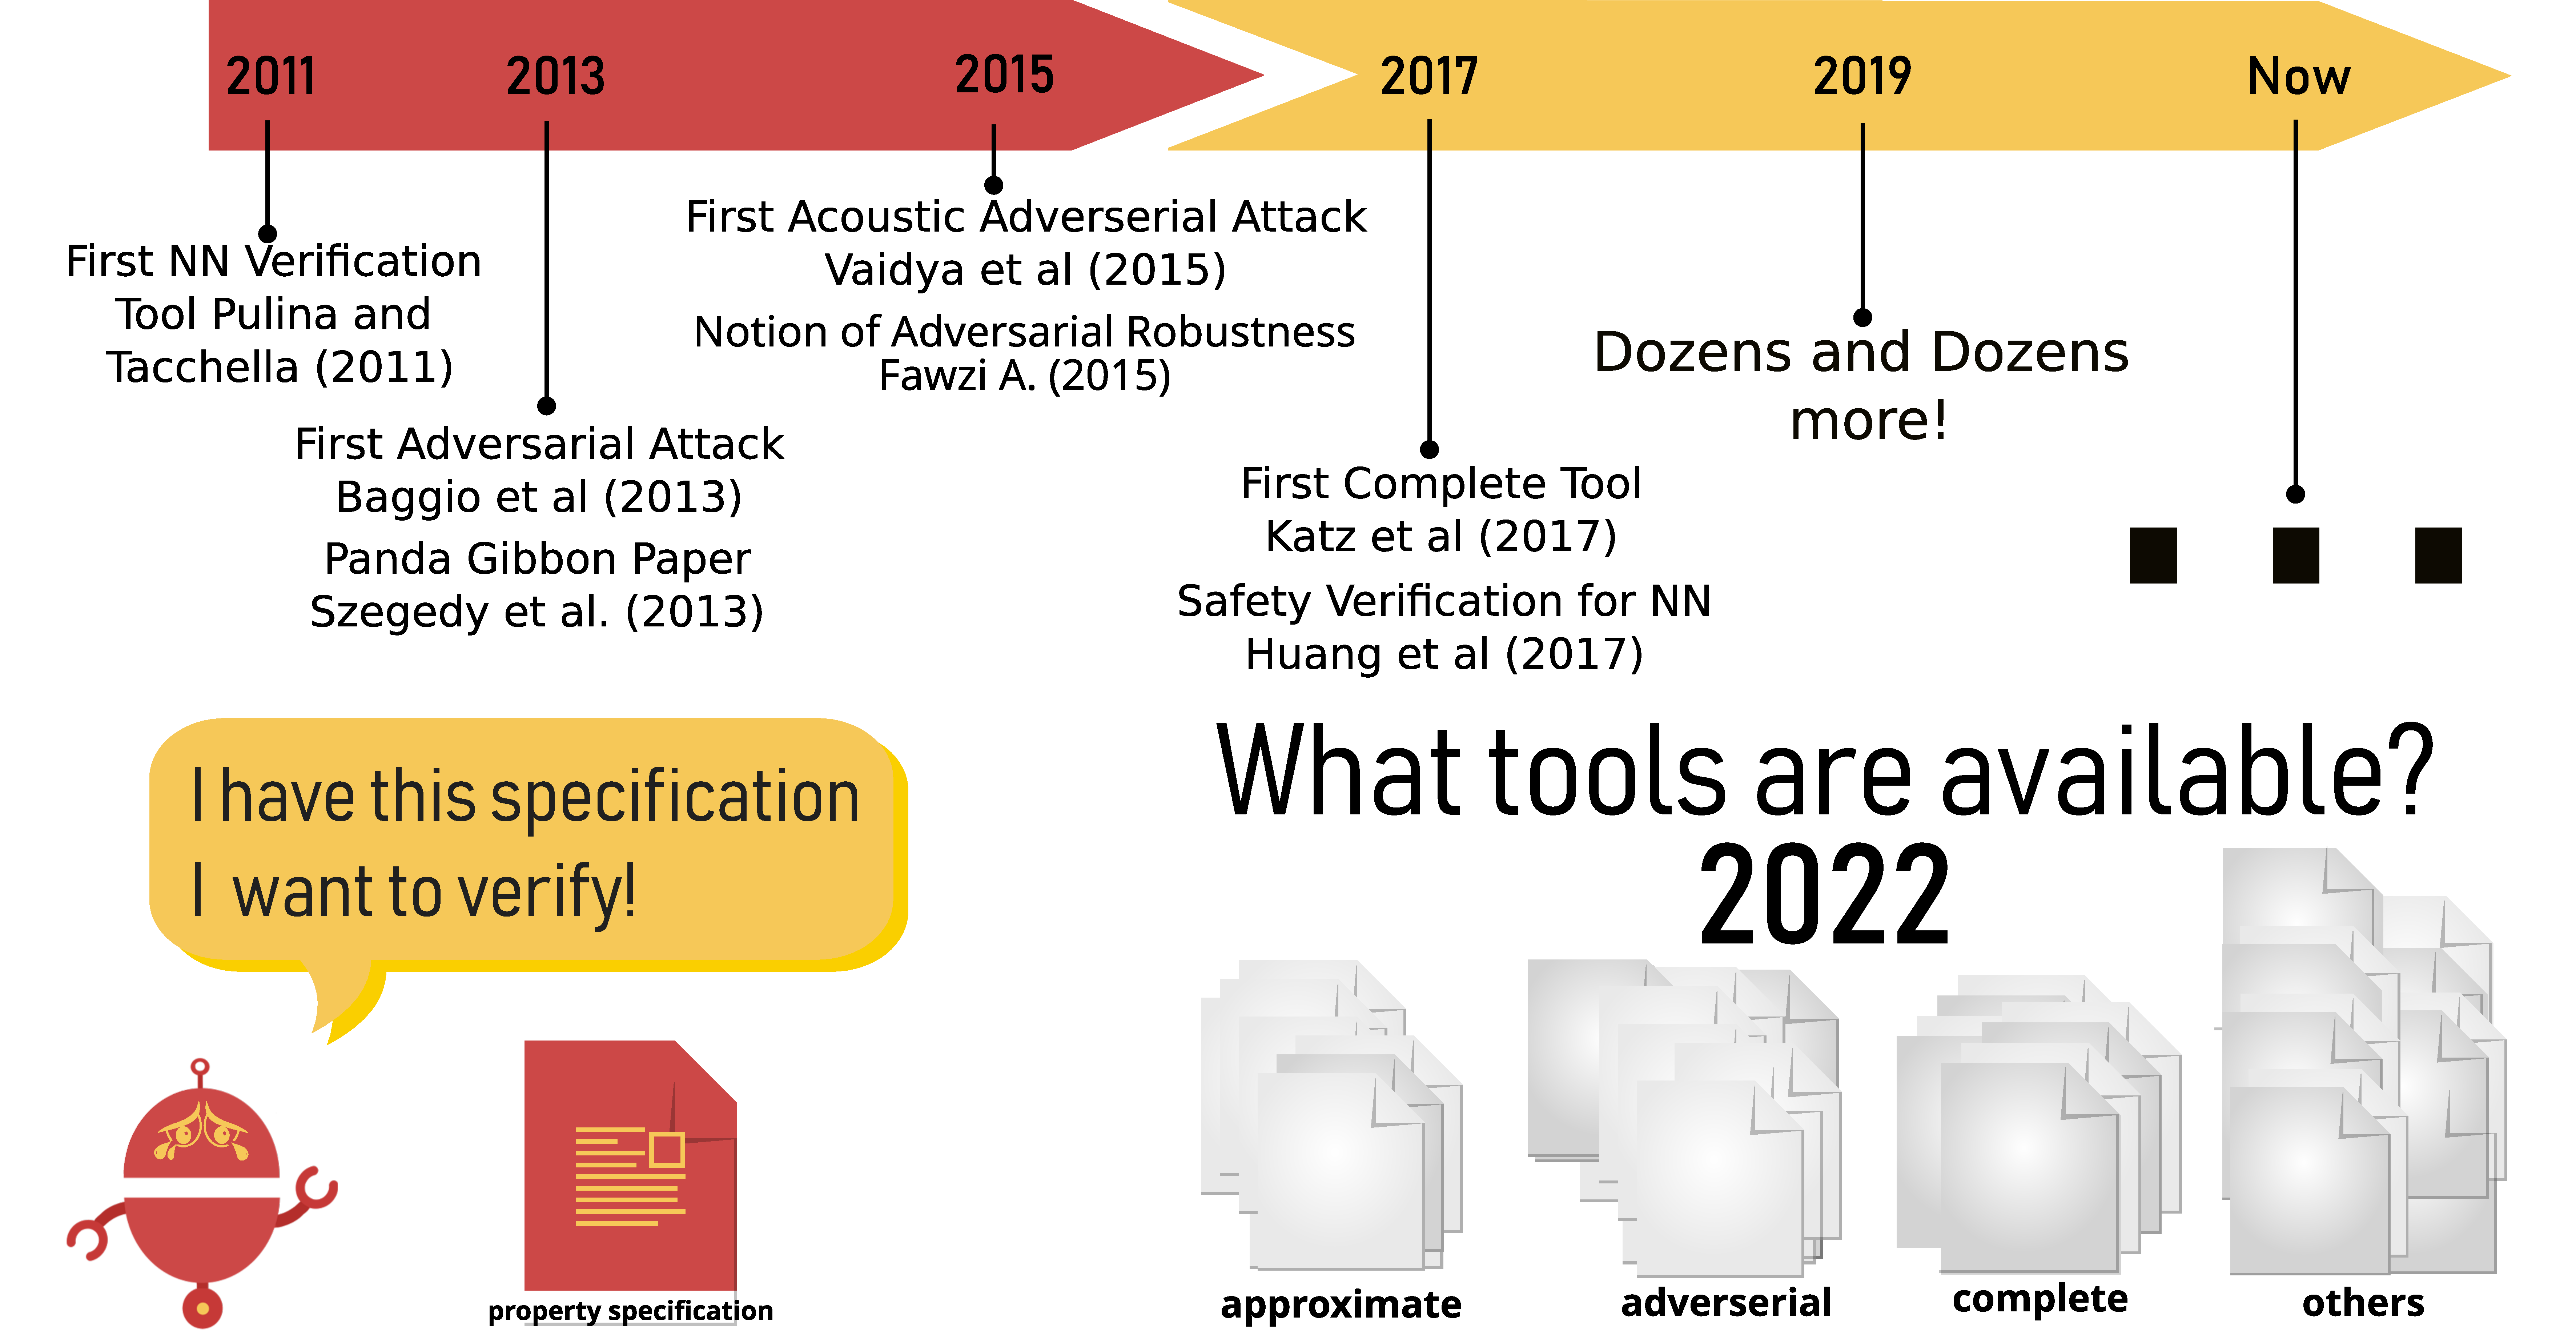
\includegraphics[width=0.9\textwidth]{Images/first-slide-2022.pdf}}
\end{frame}






\begin{frame}
\frametitle{Current Verifier Landscape}

A whole range of domain-specific verifiers exist:
\begin{itemize}
\pause
\item Marabou (SMT technology)
\pause
\item ERAN (abstract interpretation + MILP)
\pause
\item Verisig (interval arithmetic)
\item AlphaBetaCROWN (linear bound propagation)
\item $\ldots $
\end{itemize}

\begin{block}{International Standards and Competitions}
https://www.vnnlib.org/
\end{block}

\pause
Marabou is our current choice as it is complete, and the set of expressible queries is large!

  \uncover<2->{
    {\footnotesize
 \begin{thebibliography}{99}
 \beamertemplatearticlebibitems
\bibitem{1}{Guy Katz, Clarke Barrett, D. Dill, K. Julian, and M. Kochenderfer. Reluplex: An Efficient SMT Solver for Verifying Deep Neural Networks. In CAV, 2017.}
 \end{thebibliography}}}

\end{frame}

\section{The lifecycle of neural network verification}


\begin{frame}
\frametitle{The lifecycle of neural network verification}

\begin{center}
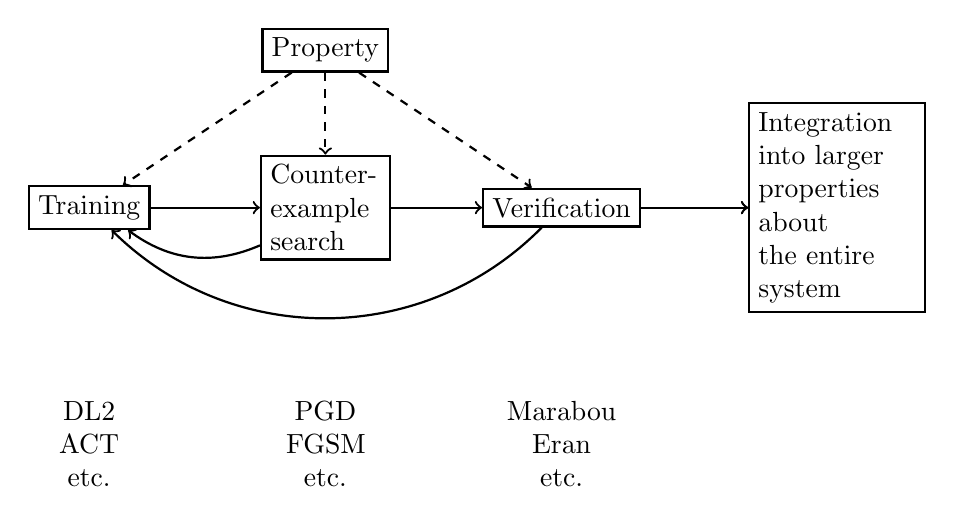
\begin{tikzpicture}[thick,
    set/.style = {circle,
        minimum size = 3cm}]

% Set A
\node[rectangle,draw] (A) at (0,4) {Property};

\onslide<2->{
\node[rectangle,draw] (B) at (-3,2) {Training};}
\onslide<3->{
\node[text width=1cm, align=center] at (-3,-1) {DL2 ACT etc.};
}

\onslide<4->{\node[rectangle,draw,text width=1.4cm] (C) at (0,2) {Counter-example search};}
\onslide<6->{
\node[text width=1cm, align=center] at (0,-1) {PGD FGSM etc.};
}

\onslide<8->{\node[rectangle,draw] (D) at (3,2) {Verification};}
\onslide<8->{
\node[text width=1.4cm, align=center] at (3,-1) {Marabou Eran etc.};
}


 \onslide<10->{\node[rectangle,draw,text width=2cm] (E) at (6.5,2) {Integration into larger properties about the entire system};
\draw [->] (D) edge (E);
}

\onslide<3->{\draw [->, dashed] (A) edge (B);}
\onslide<6->{\draw [->, dashed] (A) edge (C);}
\onslide<8->{\draw [->, dashed] (A) edge (D);}

\onslide<4->{\draw [->] (B) edge (C);}
\onslide<8->{\draw [->] (C) edge (D);}
\onslide<10->{\draw [->] (D) edge (E);}

\onslide<7->{\draw [->] (C) edge[bend left] (B);}
\onslide<9->{\draw [->] (D) edge[bend left=45] (B);}
\end{tikzpicture}
\end{center}
\end{frame}

\section{Challenges and Languages}

\begin{frame}
  \frametitle{Challenges the area faces}

  \begin{itemize}[<+->]
  \item Theory: finding appropriate verification properties
\item  Solvers: undecidability of non-linear real arithmetic  and scalability of neural network verifiers
\item ML: understanding and integrating property-driven training

\item Programming: finding the right languages to support these developments
\item Complex systems: integration of neural net verification into complex systems
  \end{itemize}
\end{frame}

\begin{frame}
\frametitle{}
  \begin{alertblock}{Some of these problems are aggravated by insufficient
  programming language or API support}

Lets look under the hood...
  \end{alertblock}

 % \begin{block}{}
%\end{block}
    \end{frame}

\begin{frame}
\frametitle{Training framework: DL2}

%\only<1>{
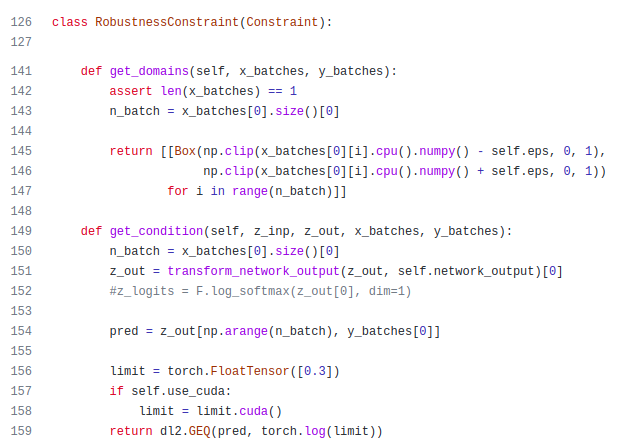
\includegraphics[width=0.9\linewidth]{Images/DL2.png}
%}

%\only<2>{
%\begin{equation*}
%\forall x : \distance{x}{\hat{x}} \leq \epsilon \Rightarrow \distance{f(x)}{f(\hat{x})} \leq \delta
%\end{equation*}
%}

  \uncover<1->{
    {\scriptsize
 \begin{thebibliography}{99}
 \beamertemplatearticlebibitems
\bibitem{1}{Fischer, M., Balunovic, M., Drachsler-Cohen, D., Gehr, T., Zhang, C., and
Vechev, M. T.
DL2: training and querying neural networks with logic.
In Proc. of the 36th Int. Conf. Machine Learning, ICML 2019}
 \end{thebibliography}}}

\end{frame}

\begin{frame}
\frametitle{Training framework: ART}
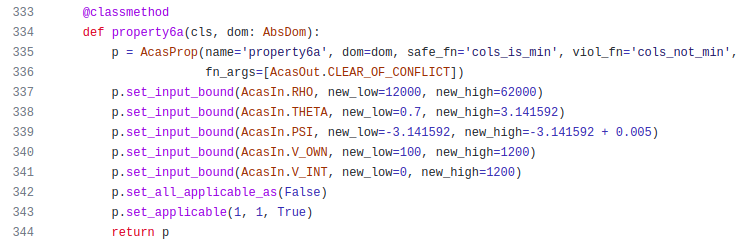
\includegraphics[width=1\linewidth]{Images/art.png}

  \uncover<1->{
    {\scriptsize
 \begin{thebibliography}{99}
 \beamertemplatearticlebibitems
\bibitem{1}{Lin, X., Zhu, H., Samanta, R., and Jagannathan, S. (2020).
Art: Abstraction refinement-guided training for provably correct neural
networks.
In FMCAD 2020}
 \end{thebibliography}}}
\end{frame}

\begin{frame}
\frametitle{Verification framework: Marabou }
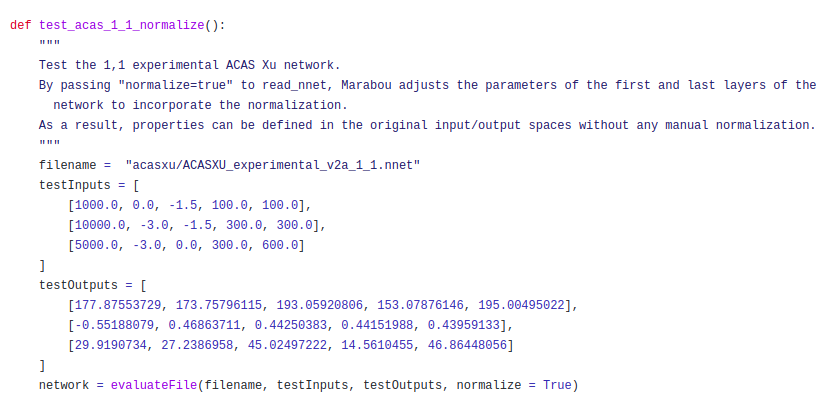
\includegraphics[width=0.9\linewidth]{Images/marabou.png}

  \uncover<1->{
    {\scriptsize
 \begin{thebibliography}{99}
 \beamertemplatearticlebibitems
\bibitem{1}{Katz, G., Huang, D. A., Ibeling, D., Julian, K., Lazarus, C., Lim, R., Shah, P.,
Thakoor, S., Wu, H., Zeljic, A., Dill, D. L., Kochenderfer, M. J., and Barrett,
C. W. (2019).
The Marabou framework for verification and analysis of deep neural
networks.
In CAV 2019}
 \end{thebibliography}}}
\end{frame}

\begin{frame}
\frametitle{Verification framework: ERAN}
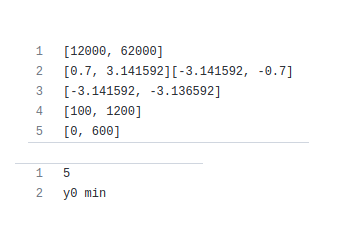
\includegraphics[width=0.5\linewidth]{Images/eran.png}

 \uncover<1->{
    {\scriptsize
 \begin{thebibliography}{99}
 \beamertemplatearticlebibitems
\bibitem{1}{Singh, G., Gehr, T., Püschel, M., and Vechev, M. T. (2019).
An abstract domain for certifying neural networks.
PACMPL, 3(POPL):41:1–41:30.}
 \end{thebibliography}}}
\end{frame}

\begin{frame}
\frametitle{Verification property language: VNNLIB}
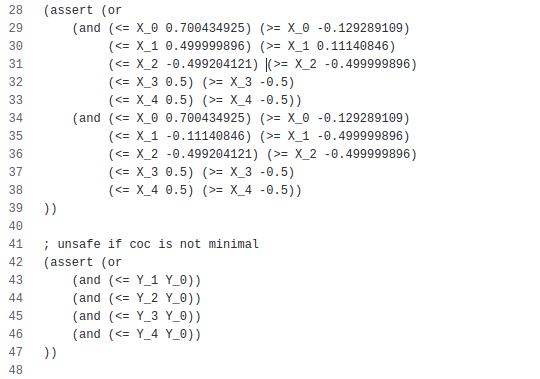
\includegraphics[width=0.8\linewidth]{Images/vnnlib.png}
\end{frame}




\begin{frame}
\frametitle{Recap: What are the problems from the PL perspective?}

\pause
\begin{itemize}
\item[$I^O$] Interoperability -- properties are not portable between training/counter-example search/ verification.
\pause
\item[$I^{P}$] Interpretability -- code is not easy to understand.
\pause
\item[$I^{\int}$] Integration -- properties of networks cannot be linked to larger control system properties.
\pause
\item[$E^G$] Embedding gap -- little support for translation between problem space (as in original spec) and input space (at neural network level).
\end{itemize}

\alert{Vehicle is designed to address all of these problems}

\end{frame}

\begin{frame}
\frametitle{Vehicle ...}

 \textbf{ is a domain-specific functional language for writing high-level property specifications for neural networks}

\begin{center}
\begin{tikzpicture}[thick,
    set/.style = {circle,
        minimum size = 3cm}]

% Set A
\node[rectangle,draw] (A) at (1.5,5) {\alert<1->{Property in Vehicle}};

\node[rectangle,draw] (B) at (-3,2) {\alert<4->{Training}};
\node[text width=1cm, align=center] at (-3,0) {\alert<4->{DL2 or other DL (native)}};

\node[rectangle,draw, dashed,text width=1.4cm] (C) at (0,2) {\alert<5->{Counter-example search}};
\node[text width=1cm, align=center] at (0,0) {\alert<5->{PGD FGSM etc.}};

\node[rectangle,draw] (D) at (3,2) {\alert<3->{Verification}};
\node[text width=1.4cm, align=center] at (3,0) {\alert<3->{Marabou} Eran etc.};

\node[rectangle,draw] (E) at (6,2) {\alert<6->{Integration}};
\node[text width=2cm, align=center] at (6,-0.3) {\alert<6->{Agda} Imandra KeymaeraX etc.};

\draw [->] (A) edge (B);
\draw [->, dashed] (A) edge (C);
\draw [->] (A) edge (D);
\draw [->] (A) edge (E);
%\draw [->, dashed] (A) edge (C);
\draw [->, dotted] (B) edge (C);
\draw [->, dotted] (C) edge (D);
\draw [->, dotted] (D) edge (E);

\onslide<1->{
\node[rectangle,draw,fill=normal text.bg] (D) at (1.5,4) {\alert<2->{Analysis \& informative error messages}};
}


\end{tikzpicture}
\end{center}
\end{frame}

\begin{frame}
\frametitle{Other Similar APIs}
\footnotesize{
\begin{itemize}%[<+->]

\item Socrates [in Python]:  Given a spec and a network (in JSON), calls different NN verifiers.
  {\scriptsize
 \begin{thebibliography}{99}
 \beamertemplatearticlebibitems
\bibitem{1}{L. H. Pham, J. Li, and J. Sun. 2020. SOCRATES: Towards a Unified Platform for Neural Network Verification.
CoRR abs/2007.11206.}
 \end{thebibliography}}

 {\alert {\small Left unresolved: $I^O$, $I^P$, $I^{\int}$, $E^G$}}

 \pause
 \item NeVer 2.0 [in Python]: added training, prunning and quantization to this functionality.
  {\scriptsize
 \begin{thebibliography}{99}
 \beamertemplatearticlebibitems
\bibitem{1}{D. Guidotti, L. Pulina, and A. Tacchella. 2020. NeVer 2.0: Learning, Verification and Repair of Deep Neural
Networks. CoRR abs/2011.09933.}
 \end{thebibliography}}

  {\alert {\small Resolved: $I^O$ (partially). Left untesolved: $I^P$, $I^{\int}$, $E^G$ }}

 \pause
 
 \item CoCoNet [in Python]: NN format converter with GUI
  {\scriptsize
 \begin{thebibliography}{99}
 \beamertemplatearticlebibitems
\bibitem{1}{D. Guidotti, A. Tacchella, L. Pulina, S. Demarchi 2023. \url{http://neuralverification.org/}}
 \end{thebibliography}}
 
  {\alert {\small Resolved: $I^P$ (partially). Left untesolved: $I^O$, $I^{\int}$, $E^G$ }}
 
 \pause

 \item Caisar [in OCAML] -- general specification language and connection to several NN Verifiers

{\scriptsize
 \begin{thebibliography}{99}
 \beamertemplatearticlebibitems
\bibitem{1}{J. Girard-Satabin, M. Alberti, F. Bobot, Z. Chihani, and A. Lemesle. 2022. CAISAR: A platform
for Characterizing Artificial Intelligence Safety and Robustness. In AISafety.}
 \end{thebibliography}}

 {\alert {\small Resolved: $I^P$, $I^{\int}$. Left unresolved: $I^O$,  $E^G$ }}

\end{itemize}}

\end{frame}

\section{Vehicle's Role and Purpose of this Tutorial}

\begin{frame}
\frametitle{\textbf{Vehicle}'s Aim...}

\alert{... is to resolve the problems $I^O$, $I^P$, $I^{\int}$, $E^G$}
\pause

... and support community's effort towards resolution of the ``Grand Challenges"

\end{frame}

  \begin{frame}
  \frametitle{``Grand Challenges"  \& \textbf{Vehicle}}
  \footnotesize{
  \begin{itemize}
  \item Theory: finding appropriate verification properties
\item  Solvers: undecidability of non-linear real arithmetic  and scalability of neural network verifiers
\item \alert{ML: understanding and integrating property-driven training}
\item \alert{Programming: finding the right languages to support these developments}
\item \alert{Complex systems: integration of neural net verification into complex systems}
  \end{itemize}}

  \begin{center}
  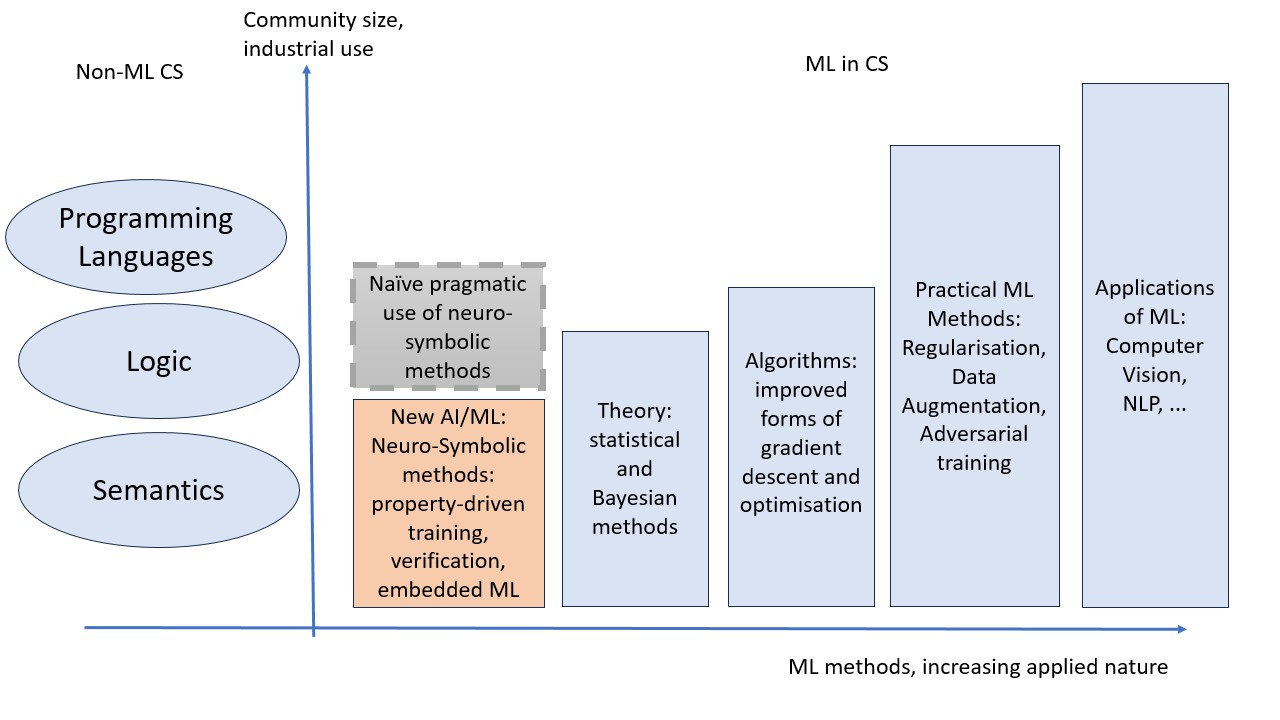
\includegraphics[scale=.20]{Images/Slide1.jpg}
  \end{center}
\end{frame}


 \begin{frame}
  \frametitle{Vehicle Architecture}
     \begin{center}
      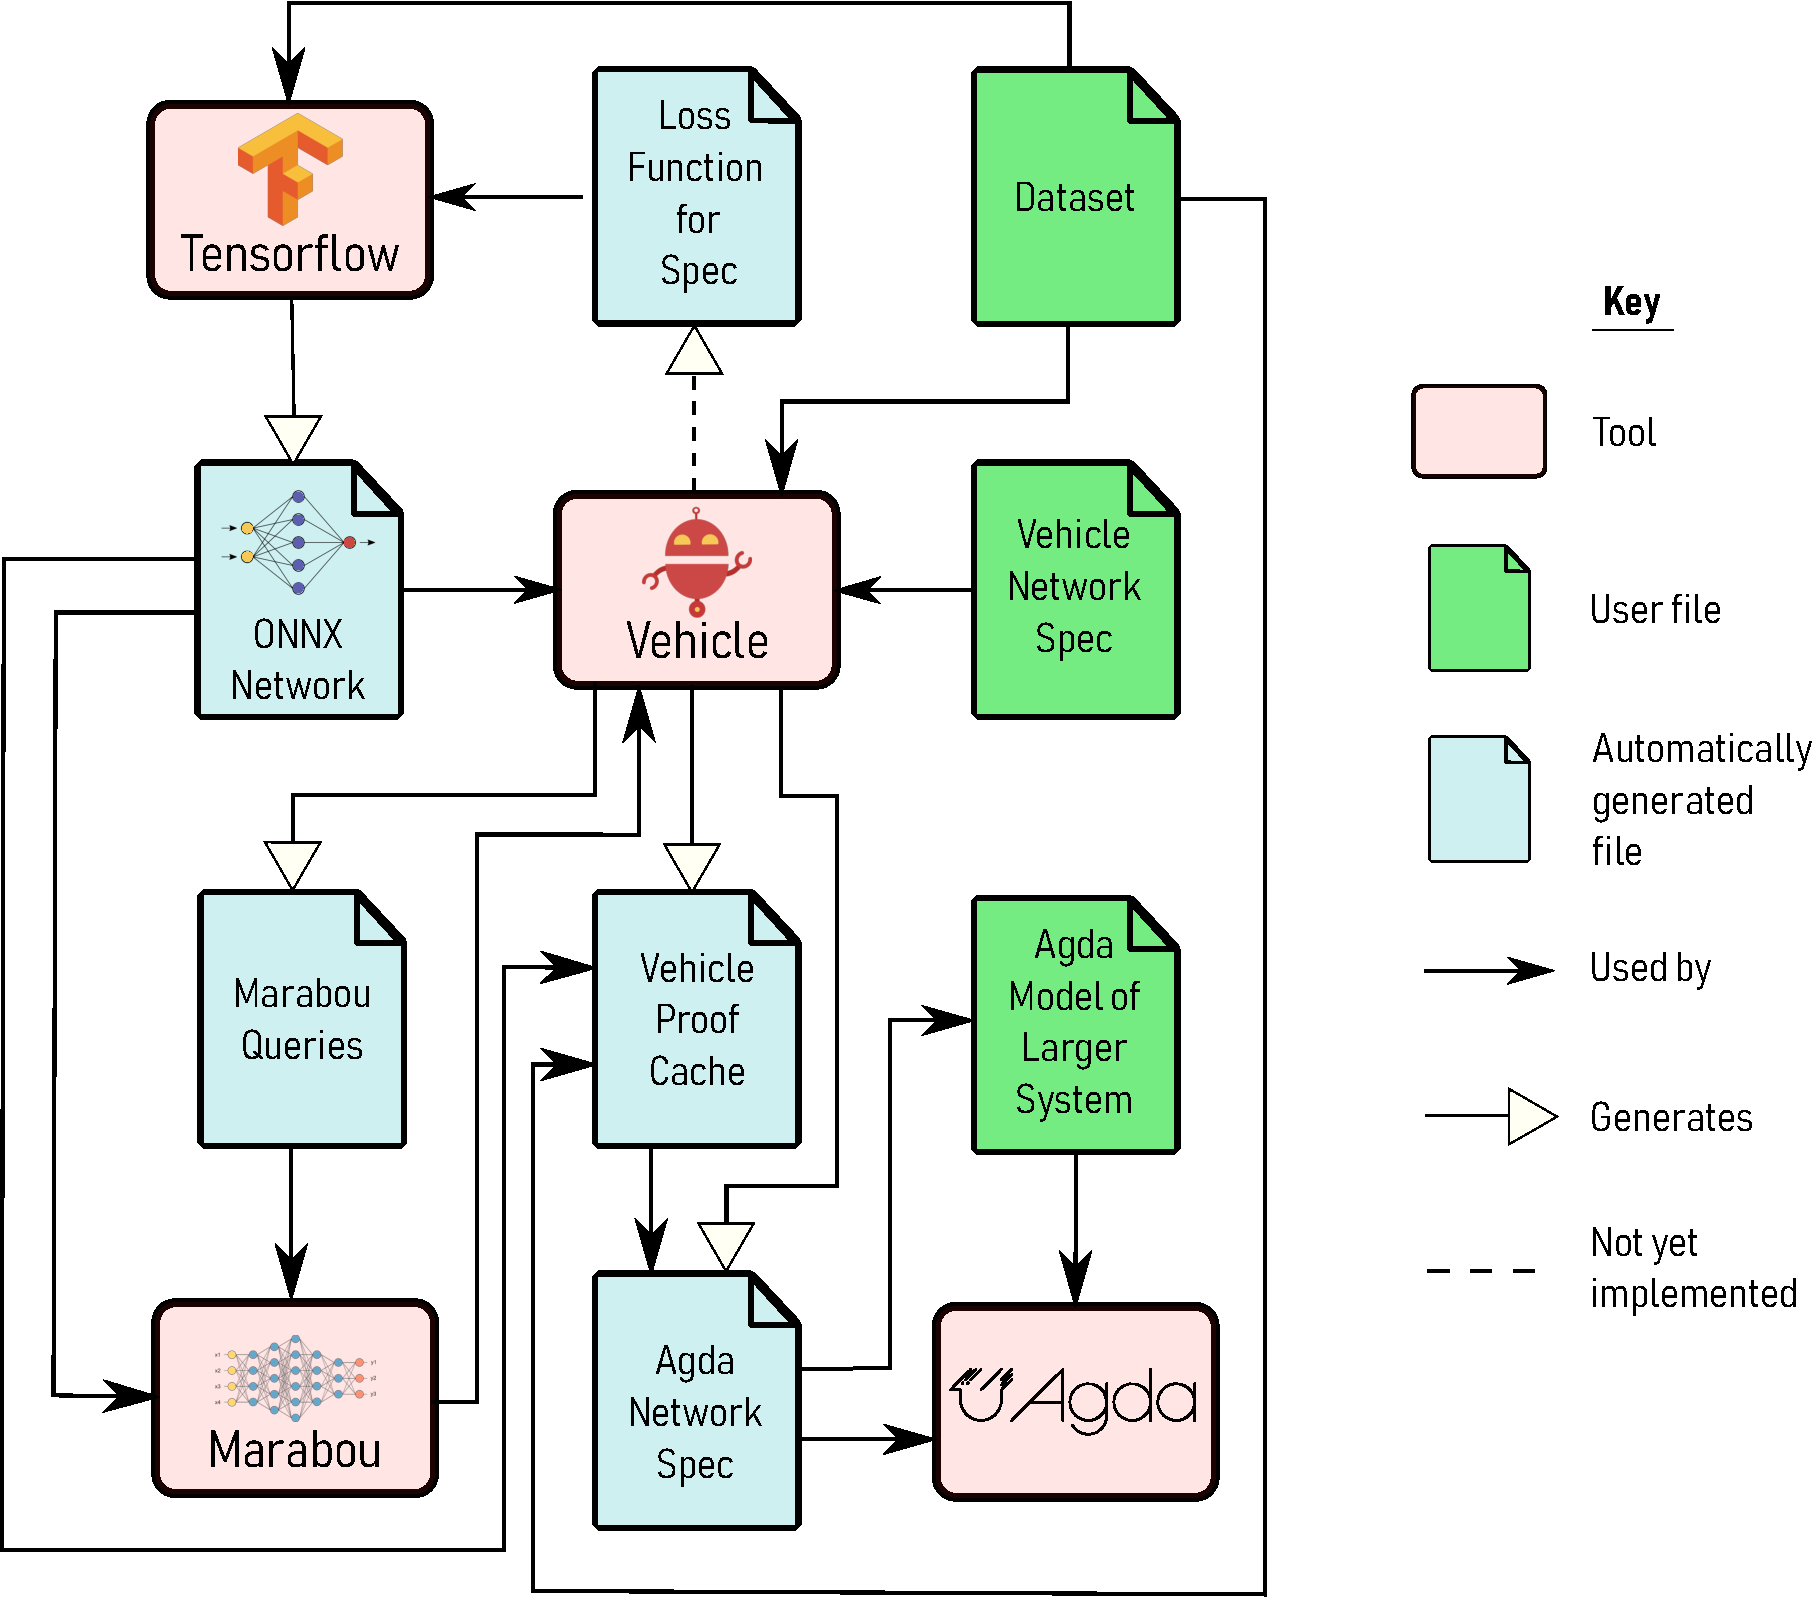
\includegraphics[scale=0.25]{Images/full-architecture-fixed}
    \end{center}

  \end{frame}

\begin{frame}
\frametitle{Sources}

    {\scriptsize
 \begin{thebibliography}{99}
 \beamertemplatearticlebibitems
\bibitem{1}{M. Daggitt, R. Atkey, W. Kokke, E. Komendantskaya, L. Arnaboldi:
Compiling Higher-Order Specifications to SMT Solvers: How to Deal with Rejection Constructively. CPP 2023}

\bibitem{2}{N. Slusarz, E. Komendantskaya, M. Daggitt, R. Stewart, K. Stark:
Logic of Differentiable Logics: Towards a Uniform Semantics of DL. LPAR 2023.}

\bibitem{3}{
 	Matthew L. Daggitt, Wen Kokke, Robert Atkey, Luca Arnaboldi, Ekaterina Komendantskaya:
Vehicle: Interfacing Neural Network Verifiers with Interactive Theorem Provers. FOMLAS 2022}

\bibitem{4}{Vehicle Team: The Vehicle language: \url{https://github.com/vehicle-lang} 2023.}

\bibitem{5}{M.Daggitt and W.Kokke: Vehicle User Manual. \url{https://vehicle-lang.readthedocs.io} 2023.}

\bibitem{6}{The Vehicle team: Vehicle Tutorial \url{https://vehicle-lang.github.io}. 2023. Tutorial code repository \url{https://github.com/vehicle-lang/vehicle-tutorial}. }
 \end{thebibliography}}

\end{frame}

\begin{frame}
\frametitle{Purpose of this Tutorial...}

\begin{block}{}
\begin{itemize}
\item Introduce \textbf{Vehicle} specification language at the user level
\item Discuss challenges in NN verification ("grand" and technical)
\item Gather feedback and obtain community support
\end{itemize}
\end{block}

\begin{block}{Thanks}
... to Marabou team and FOMLAS organisers for the continuing support!
\end{block}
\end{frame}

\begin{frame}
\frametitle{Plan for the rest of this tutorial}

\begin{itemize}
\item Before coffee break:
\begin{itemize}
\item Brief introduction to \textbf{Vehicle} specification language 
\item \alert{Exercise session:} write and verify a spec (with possibility to extend over the break

Requirements (see also "Prerequisites" \url{https://vehicle-lang.github.io}): 

\begin{itemize}
\item for writing a spec, install vehicle: just run 

\texttt{pip install vehicle}

\item for verifying a spec, you also need Marabou installed (see Marabou pages)
\end{itemize}
\end{itemize}
\item After the break:
\begin{itemize}
\item Demo of property-driven training in Vehicle 
\item Demo of large system integration in Vehicle
\end{itemize}

\item After this tutorial -- Natalia Slusarz: theory behind property-driven training
\end{itemize}

\end{frame}


\end{document}


\section{Introduction to Vehicle}

\begin{frame}[fragile]
\frametitle{Types}
Let us build the ACAS Xu specification.

We start with types of input and output vectors, as well as types of ACAS Xu networks

\begin{minted}[fontsize=\small]{vehicle}

type InputVector = Vector Rat 5
type OutputVector = Vector Rat 5

@network
acasXu : InputVector -> OutputVector
\end{minted}

\begin{block}{}

The Vector type represents a mathematical vector, or in programming terms can be thought of as a fixed-length array.
\end{block}
\end{frame}

\begin{frame}[fragile]
\frametitle{Values}

Types for values are automatically inferred by \textbf{Vehicle}. For example, we can declare the number $\pi$ and its type will be inferred as rational:

\begin{minted}[fontsize=\small]{vehicle}

pi = 3.141592
\end{minted}
\end{frame}

\begin{frame}[fragile]
\frametitle{Working with vectors}
\begin{itemize}
\item some input or output pre-processing maybe expected when defining a neural network.

\begin{example}
It is assumed that the ACAS Xu inputs and outputs are normalised, i.e. the network does not work directly with units like $m/s$. However, the specifications  we want to write should ideally concern the original units.
\end{example}

\pause

\item This is an instance of \emph{`` problem space / input space mismatch"}
\item ... that is very common in neural net verification

\item
Being able to reason about problem space (alongside the input space) is a feature that distinguishes \textbf{Vehicle} from
majority of the mainstream neural network verifiers
\end{itemize}
\end{frame}

\begin{frame}[fragile]
\frametitle{Vector normalisation}
For clarity, we define a new type synonym for unnormalised input vectors which are in the problem space.
\begin{minted}[fontsize=\footnotesize]{vehicle}

type UnnormalisedInputVector = Vector Rat 5

\end{minted}

Next we define the range of the inputs that the network is designed
to work over.

\begin{minted}[fontsize=\footnotesize]{vehicle}

minimumInputValues : UnnormalisedInputVector
minimumInputValues = [0,0,0,0,0]

maximumInputValues : UnnormalisedInputVector
maximumInputValues = [60261.0, 2*pi, 2*pi, 1100.0, 1200.0]

meanScalingValues : UnnormalisedInputVector
meanScalingValues = [19791.091, 0.0, 0.0, 650.0, 600.0]
\end{minted}
\end{frame}

\begin{frame}[fragile]
\frametitle{Vector manipulation}
An alternative method to vector definition is to use the `foreach` constructor, which is used to provide a value for each `index i`.
\begin{minted}[fontsize=\footnotesize]{vehicle}

minimumInputValues : UnnormalisedInputVector
minimumInputValues = foreach i . 0

\end{minted}
Let us see how  `foreach` works with vector indexing.

We can now define the normalisation function that takes an input vector and
returns the unnormalised version.

\begin{minted}[fontsize=\footnotesize]{vehicle}

normalise : UnnormalisedInputVector -> InputVector
normalise x = foreach i .
  (x ! i - meanScalingValues ! i) / (maximumInputValues ! i)
\end{minted}

\pause
... our first acquaintance with functions!

\end{frame}

\begin{frame}[fragile]
\frametitle{Functions and types}
\begin{minted}[fontsize=\footnotesize]{vehicle}
<name> : <type>
<name> [<args>] = <expr>

\end{minted}
Functions make up the backbone of the \textbf{Vehicle} language.
\pause
\begin{minted}[fontsize=\footnotesize]{vehicle}

validInput : UnnormalisedInputVector -> Bool
validInput x = forall i .
  minimumInputValues ! i <= x ! i <= maximumInputValues ! i

\end{minted}

\pause

\begin{block}{Our first acquaintance with quantifiers!}
 One of the main advantages of \textbf{Vehicle} is that it can be used to state and prove specifications that describe the network’s behaviour over an infinite set of values.
\end{block}

\end{frame}


\begin{frame}[fragile]
\frametitle{Functions and types}

\begin{block}{Function Composition: Exercise!}
\begin{minted}[fontsize=\footnotesize]{vehicle}
normAcasXu : UnnormalisedInputVector -> OutputVector
normAcasXu x = acasXu (normalise x)
\end{minted}
\end{block}

\end{frame}

\begin{frame}[fragile]
\frametitle{Pre-defined functions and predicates}
We have already used:
\begin{minted}[fontsize=\footnotesize]{vehicle}
*
/
!
<=
\end{minted}

\begin{block}{Exercise}
\footnotesize{What do they stand for?}
\end{block}
\end{frame}

\begin{frame}[fragile]
\frametitle{Lets verify ACAS Xu!}
\begin{minted}[fontsize=\footnotesize]{vehicle}
distanceToIntruder = 0   -- measured in metres
angleToIntruder    = 1   -- measured in radians
intruderHeading    = 2   -- measured in radians
speed              = 3   -- measured in metres/second
intruderSpeed      = 4   -- measured in meters/second

clearOfConflict = 0
weakLeft        = 1
weakRight       = 2
strongLeft      = 3
strongRight     = 4
\end{minted}
\footnotesize{
The fact that all vector types come annotated with their size means that it
 is impossible to mess up indexing into vectors, e.g. if you changed
 `distanceToIntruder = 0` to `distanceToIntruder = 5` the specification would
 fail to type-check.}



\end{frame}

\begin{frame}[fragile]
\frametitle{Property 1}

\footnotesize{\textbf{If the intruder is distant and is significantly slower than the ownship, the score of a COC advisory will always be below a certain fixed threshold.}}

\pause

\begin{minted}[fontsize=\footnotesize]{vehicle}

intruderDistantAndSlower : UnnormalisedInputVector -> Bool
intruderDistantAndSlower x =
  x ! distanceToIntruder >= 55947.691 and
  x ! speed              >= 1145      and
  x ! intruderSpeed      <= 60
\end{minted}
\pause
\begin{block}{Exercise!}
\footnotesize{
\begin{enumerate}
\item
Can you identify whether the specification is written in terms of input space or problem space? How do you know?
\item Can you spot more pre-defined \textbf{Vehicle} functions? What are they?
\end{enumerate}}
\end{block}

\end{frame}

\begin{frame}[fragile]
\frametitle{There is little left to do!}

\footnotesize{
\textbf{If the intruder is distant and is significantly slower than the ownship, the score of a COC advisory will always be below a certain fixed threshold.}}

\pause

\begin{minted}[fontsize=\footnotesize]{vehicle}
@property
property1 : Bool
property1 = forall x .
   validInput x and intruderDistantAndSlower x =>
           normAcasXu x ! clearOfConflict <= 1500
\end{minted}
\pause
\begin{block}{Exercise!}
\footnotesize{
\begin{enumerate}
\item Can you guess the purpose of the syntax
\begin{minted}{vehicle}
@property
\end{minted}
?
\item What kind of domain  `forall` ranges over? Is it finite or infinite?
\end{enumerate}}
\end{block}

\end{frame}

\begin{frame}[fragile]
\frametitle{How to run Vehicle}
\begin{block}{Checklist}
\begin{enumerate}
\item a verifier installed (Marabou);
\item the actual network is supplied in an ONNX format
\item \textbf{Vehicle} is installed.
\end{enumerate}
\end{block}

\pause
\begin{minted}[fontsize=\footnotesize]{vehicle}
vehicle --compileAndVerify
  --specification acasXu.vcl
  --verifier Marabou
  --network acasXu:acasXu_1_7.onnx
  --property property1

--------------------------------------------------
Verifying properties:
  property1 [===========================] 1/1 queries complete
Result: true
   property1
\end{minted}
\end{frame}

\begin{frame}[fragile]
\frametitle{Exercise: $\epsilon$-ball Robustness}
 \begin{minted}[fontsize=\tiny]{vehicle}
type Image = Tensor Rat [28, 28]
type Label = Index 10
validImage : Image -> Bool
validImage x = forall i j . 0 <= x ! i ! j <= 1

@network
classifier : Image -> Vector Rat 10

advises : Image -> Label -> Bool
advises x i = forall j . j != i => classifier x ! i > classifier x ! j

@parameter
epsilon : Rat

boundedByEpsilon : Image -> Bool
boundedByEpsilon x = forall i j . -epsilon <= x ! i ! j <= epsilon

robustAround : Image -> Label -> Bool
robustAround image label = forall pertubation .
  let perturbedImage = image - pertubation in
  boundedByEpsilon pertubation and validImage perturbedImage =>
    advises perturbedImage label

@dataset
trainingImages : Vector Image n

@dataset
trainingLabels : Vector Label n

@property
robust : Vector Bool n
robust = foreach i . robustAround (trainingImages ! i) (trainingLabels ! i)
\end{minted}
\end{frame}

\begin{frame}
\frametitle{Vehicle ...}

 \textbf{ is a domain-specific functional language for writing high-level property specifications for neural networks}

\begin{center}
\begin{tikzpicture}[thick,
    set/.style = {circle,
        minimum size = 3cm}]

% Set A
\node[rectangle,draw] (A) at (1.5,5) {\alert{\textbf{Property in Vehicle}}};

\node[rectangle,draw] (B) at (-3,2) {Training};
\node[text width=1cm, align=center] at (-3,0) {DL2 ACT etc.};

\node[rectangle,draw,text width=1.4cm] (C) at (0,2) {Counter-example search};
\node[text width=1cm, align=center] at (0,0) {PGD FGSM etc.};

\node[rectangle,draw] (D) at (3,2) {\alert{\textbf{Verification}}};
\node[text width=1.4cm, align=center] at (3,0) {\alert{\textbf{Marabou}} Eran etc.};

\node[rectangle,draw] (E) at (6,2) {Integration};
\node[text width=2cm, align=center] at (6,-0.3) {Agda Imandra KeymaeraX etc.};

\draw [->, dashed] (A) edge (B);
\draw [->, dashed] (A) edge (C);
\draw [->, dashed] (A) edge (D);
\draw [->, dashed] (A) edge (E);

\draw [->] (B) edge (C);
\draw [->] (C) edge (D);
\draw [->] (D) edge (E);

\onslide<1->{
\node[rectangle,draw,fill=normal text.bg] (D) at (1.5,4) {\alert{\textbf{Analysis \& informative error messages}}};
}

\end{tikzpicture}
\end{center}
\end{frame}



\end{document}
